% 畫圖
% 處理 units 的 Gumbel 那些
% 順過

\chapter{背景知識}
\section{深層類神經網路}

\subsection{簡介}

  
深層類神經網路(Deep Neural Network,DNN)又稱「人工類神經網路(Artificial Neural Network,ANN)」,是由神經科學中連結主義(Connectionism)學派的麥氏(McCulloch)與皮氏(Pitts)等人,在 1943 年 \cite{mcculloch_logical_1943} 提出的計算模型。該學派主張藉由模仿生物神經連結的方式建立模型,以建立系統模擬各種心智現象,而其中深層類神經網路由於它在貼合目標函數上的彈性和運算上易於平行化的特徵,得以恰當利用圖形處理器(Graphics Processing Unit,GPU)等硬體裝置的優勢,能夠很好的結合最佳化演算法對貼合(Fit)資料分佈、找出最好的函數(Function),在各類任務與應用上取得前所未有的效能,因而近年為機器學習與電腦科學領域獲得重大進展,現已成為人工智慧發展的主流。

深層類神經網路最基本的單位是「神經元(Neuron)」,其本質為一個線性分類器,為了模擬生物神經細胞接收訊號、處理到傳出的過程。每個神經元會接收一串數字 \((x_1, x_2, \cdots\cdots, x_N)\) 作為輸入後,得出一個數字 \(y\) 作為輸出。其關係可用下列數學運算式描述:
$$y=\sigma(w^\top x + b) $$
其中輸入 $x = (x_1, x_2, \cdots\cdots, x_N)$ 被描述為一個 $N$ 維向量,該神經元對每個輸入取值分別給予權重(Weight) $w = (w_1, w_2, \cdots\cdots, w_N)$ 相乘後,再對加權平均的結果加上偏差值 $b$ 當成線性輸出值。最後,為了描述分類器函數的非線性(Non-linear)特性,類似神經細胞觸發與否的過程,此輸出值通常會經過激發函數(Activation Function)$\sigma$ 的轉換後才得到最終輸出值 $y$。常見的激發函數包含線性整流單元(Rectified Linear Unit,ReLU)、S 函數(Sigmoid Function)或雙曲正切函數(Hyperbolic Tangent Function,$\tanh$)等等。


\begin{figure}
    \centering
    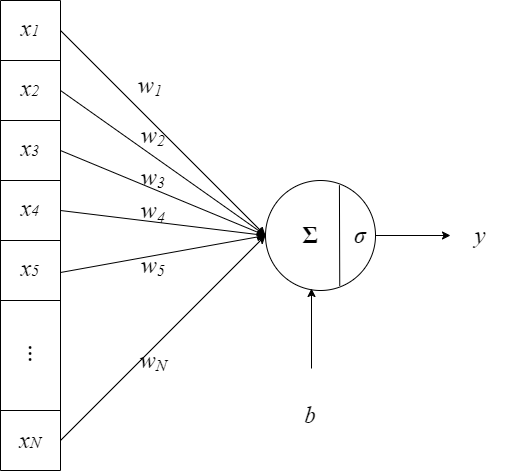
\includegraphics[width=0.5\linewidth]{figures/neuron.drawio.png}
    \caption{神經元示意圖}
    \label{fig:single-neuron}
\end{figure}

其後羅氏(Rosenblatt)在 1958 年 \cite{rosenblatt_perceptron_1958} 提出感知器(Perceptron),本質上是結合數個神經元的運算,來實現更為複雜的函數功能。基於數學理論中的通用近似定理(Universal Approximation Theorem)\cite{funahashi_approximate_1989},感知器理想上可以近乎模擬一切函數。然而後續研究發現單層感知器具有線性不可分\footnote{例如無法貼合異或(Exclusive OR,XOR)運算等函數}的限制,於是出現了在輸入與輸出函數之間增加隱藏層(Hidden Layer)的多層感知器(Multi-layered Perceptron,MLP),由於在輸入與輸出之間的多層感知器可以藉助隱藏層的幫助實現函數的多次轉換,因而大大拓展了模型的適用範圍。此種計算模型由於是「加深隱藏層」得來的,因而被稱為深層類神經網路(Deep Neural Network)。

然而,單純擁有能夠表達複雜函數的模型是不夠解決現實複雜的工程問題的。為了找出資料所描述的函數,類神經網路會藉由計算輸出層與目標函數之間的誤差(Error),透過最佳化演算法計算出梯度(Gradient)後,逐步逼近由資料集呈現的函數,此過程稱為梯度下降法(Gradient Descent),可寫為:
$$\theta_{t+1} \leftarrow \theta_{t} - \eta \nabla_\theta\mathcal{L}(\mathcal{D}, f_{\theta_t}(\cdot))$$
其中 $t$ 為當前的迭代數,$\theta_t$ 為當前模型參數,$\theta_{t+1}$ 為更新後之模型參數。$\mathcal{D}$ 是資料集,將與模型參數 $\theta$ 形成的函數 $f_\theta$ 之間透過減損函數(Loss Function)$\mathcal{L}$ 計算出誤差,求得對 $\theta$ 的梯度後以學習率(Learning Rate)$\eta$ 為倍率對整個進行更新。

為了增加函數貼合的效率,魯氏(Rumelhart)與辛氏(Hinton)等人 \cite{rumelhart_learning_1986, rumelhart_learning_1987} 提出了反向傳播(Backpropagation)演算法,期望將上述更新網路的學習過程,經由隱藏層反向往輸入層,對整個類神經網路進行修正。配合圖形處理器平行運算的能力,資料中貼合函數的過程變得更有效率。如此透過深層類神經網路,找出資料輸入與輸出之間的函數關係的機器學習演算法,就稱之為深層學習(Deep Learning)。由於深層學習的可擴展性(Scalibility)與泛用性(Generalizability),不論在圖像、語音、文字等多個模態,深層類神經網路都已經獲得了廣泛應用,解決更加複雜的現實問題。

實際上,根據資料特性的不同,並不是所有的資料都能單純的適用於這類輸入與輸出向量直接對應的模式,因此類神經網路又發展出不同的架構以適應資料本身的特性。前述的類神經網路由於運算過程單純是從輸入層經由多層感知器直接進行矩陣運算完成函數的模擬,因此被稱之為「前饋式類神經網路(Feed Forward Network,FFN)」。為了適應各種資料型態的特徵,藉由調整各神經元之間的連接關係,後續發展出了如卷積式(Convolutional)、遞迴式(Recurrent)與轉換器(Transformer)類神經網路等架構,以應對不同任務的需求。由於這些架構在語音與文字處理上相當常用,接下來將一一分別介紹:

\subsection{卷積式類神經網路}

  
卷積式類神經網路(Convolutional Neural Network,CNN)為 1998 年由楊氏(LeCun) \cite{lecun_gradient-based_1998} 提出,旨在利用訊號處理上卷積(Convolution)的運算模擬人類視覺皮質感知 \cite{hubel_receptive_1959} 的特性,利用其移動不變性(Shift-invariance)來捕捉二維影像中的局部(Local)特徵,以便後續的類神經網路可以對輸入的資料進行更整體而全面的判斷。

有別於圖像中經常是以像素 (Pixel)的三原色亮度進行卷積運算,在語音中卷積式類神經網路的處理對象,除了直接是空氣壓力波形的物理訊號以外,為了更方便機器模型判斷語音訊號的內容,透過聲學知識得到的聲學特徵或深層學習得出的語音表徵,也經常是語音處理中卷積層運算的對象。然而不論是何種輸入,有別於影像的二維資料,語音訊號的資訊是被呈現在時間軸的維度上,因此除了使用影像的二維卷積運算,也會出現一維的卷積式類神經網路,以模仿人耳聽覺對時變訊號的窗框(Window)處理過程,讓模型可以觀察到輸入語音在不同解析度(Resolution)上的資訊,例如本研究特別著重的音位(Phoneme)等。


\subsection{遞迴式類神經網路與序列至序列(Sequence-to-sequence,Seq2seq)模型}

\subsubsection{遞迴式類神經網路}

  
不同於運算過程由輸入往輸出單向的前饋式和卷積式類神經網路,為了處理有記憶和狀態的資料,特別是會隨時間變化的序列資訊,在語音和文字的機器學習中,會將輸出訊號重新接回輸入層的遞迴式類神經網路(Recurrent Neural Network,RNN)是一個相當符合語言特性的選擇。此種網路以每個時間點(Timestep)為考慮對象,在每一步會對輸入層的向量進行運算後,不但將此結果算出一個輸出向量,還會得到另外一些數據保留作內部狀態,表示此前經歷過所有序列資料的記憶。常用的遞迴式類神經網路類型有長短期記憶(Long Short-term Memory,LSTM)和閘門循環單元(Gated Recurrent Unit,GRU)等。
  
此類類神經網路通常會以下列介紹的序列至序列的形式被用在如語音辨識、語音合成或機器翻譯等和語言密切相關的任務中。

\subsubsection{序列至序列(Sequence-to-sequence,Seq2seq)模型}

  
由於許多以語言為主的資料經常以兩個序列互相配對的形式呈現,因此專門用以處理此類資料的模型被特別稱為序列至序列模型。此類模型一般的架構是由一個編碼器(Encoder)和一個解碼器(Decoder)構成,旨在模擬輸入與輸出序列之間的變化與相依關係(Dependency)。

此類模型一般有兩種模式:其一是每個時間點都取得一個輸出的向量,用在輸入與輸出等長的任務之中,此模式又被稱為符記分類(Token Classification);但更常見的狀況是,輸入與輸出兩者序列長度並不總是相同,此時典型的作法是,讓編碼器將輸入序列在每個時間點一一與模型進行運算,藉由內部表徵(Latent Representation)的調整對整個輸入序列進行編碼,完成後將最後一個時間點的表徵作為整個序列的代表,此表徵向量會被稱為「語境向量(Context Vector)」,接著被傳遞給解碼器依時序生成輸出訊號的序列。

\subsection{專注機制(Attention Mechanism)與轉換器(Transformer)類神經網路}

\subsubsection{專注機制}

  
由於遞迴式類神經網路本身需要編碼和解碼的資訊量是整個序列,對時間點距離比較遠的輸入容易被遺忘,也就是難以處理長期相依性(Long-term Dependency)的問題。為解決這種困境,巴氏(Bahdanau)等人提出了「專注機制(Attention mechanism)」\cite{bahdanau2014neural},讓解碼器將每一個輸入序列的訊號皆視作「部份的」語境向量,可以對輸入序列的不同時間點的向量分配權重,使得生成輸出序列時可以依照該時間的的需求從輸入序列中得到所需的訊息。
序列至序列模型透過專注機制的引入,能夠更好的分配輸入序列的運算,因而大大改善了如語音辨識、機器翻譯等任務的效能。

\subsubsection{轉換器類神經網路}

儘管遞迴式類神經網路本身善於處理時序資料,然而它難以平行化的架構限制卻大大束縛了其在訓練和推理(Inference)時的效率。2017 年瓦氏(Vaswani) 等人 \cite{vaswani2017attention} 提出了完全由前述的專注機制構成,不需依賴遞迴運算的序列至序列模型,並稱之為「轉換器(Transformer)」,用以解決最經典的機器翻譯任務。

轉換器類神經網路一般包含編碼器和解碼器兩個部分,兩者皆為多層架構之類神經網路。以下分別對其各元件進行解說:

\paragraph{位置編碼}

對於整個編碼器或解碼器的輸入序列,模型會先以序列中不同位置的時間點進行編碼,取代原先在遞迴式類神經網路需要一步一步運算的過程,在實行平行計算的同時也能考慮到資料在不同時間點出現的效應。原先轉換器採用的是三角函數進行位置編碼,而在語音模型中的轉換器有時也會採用卷積式網路以捕捉輸入更細微的資訊。

經過位置編碼後,向量經過的每一個轉換器層(Transformer Layer)會對輸入序列進行以多頭專注為主的一連串運算:

\paragraph{多頭專注}

轉換器層中的專注機制一般涉及三個輸入向量之間:詢向量(Query)$Q$、鑰向量(Key)$K$ 和值向量(Value)$V$,隨後進行以下的專注機制運算:
\[\text{Attention}(Q, K, V) = \text{softmax}
\left(
\frac{QK^\top}{\sqrt{d_k}}
\right)
V\]
其中 $ \text{softmax}$ 為正規化指數函數 ,分母的 $d_k$  則是鑰向量 $K$ 的維度。透過此運算,每一個專注運算會透過鑰向量和詢向量內積計算專注權重,為了避免受維度過大之影響而縮小為 $\sqrt{d_k}$ 分之一後,再由正規化指數函數使得權重總和為 1 分配給值向量進行加權。

為了應對多樣的輸入訊號,每個轉換器層具備多個獨立的專注機制,會對三組輸入向量先進行各自不同的 $W^Q$、$W^K$、$W^V$ 線性轉換,稱之為「多頭專注(Multi-head Attention)」。對於第 $i$ 個專注頭(Head)便有

$$\text{head}_i = \text{Attention}(QW^Q_i,KW^K_i,VW^V_i)$$

最後,若有 $h$ 個專注頭,多頭自專注模組會將多個頭的結果進行串接(Concatenate),經過線性轉換 $W^O$ 作為模組輸出
$$\text{MultiHead}(Q, K, V) = \text{Concat}(\text{head}_1, \cdots\cdots, \text{head}_h) W^O$$

\paragraph{其他層內運算}

每一層轉換器層在經過多頭專注的運算之後,會依序進行下列三個步驟

\begin{enumerate}
\item 與輸入向量透過殘差連接(Residual Connection)相加,隨後進行層正規化(Layer Normalization)以穩定訓練
\item 將此結果通過一個簡單的前饋式類神經網路對向量做線性轉換
\item 再將前饋網路的輸入與輸出再次計算殘差總和後,進行層正規化輸出
\end{enumerate}

以上為轉換器被提出時的最原始模型,其後對殘差連接、層正規化的安排也存在各類變體。

\paragraph{跨專注機制}

由於解碼器相較於編碼器,需要來自編碼器輸入序列的資訊幫助輸出。因此,原本在編碼器層中的自專注機制,在解碼器會再經過一次跨專注機制的運算,改為使用編碼器提供的詢向量和鑰向量對解碼器的值向量做專注運算。

圖 \ref{fig:tfm_arch} 是完整的轉換器整體架構圖:
\begin{figure}
    \centering
    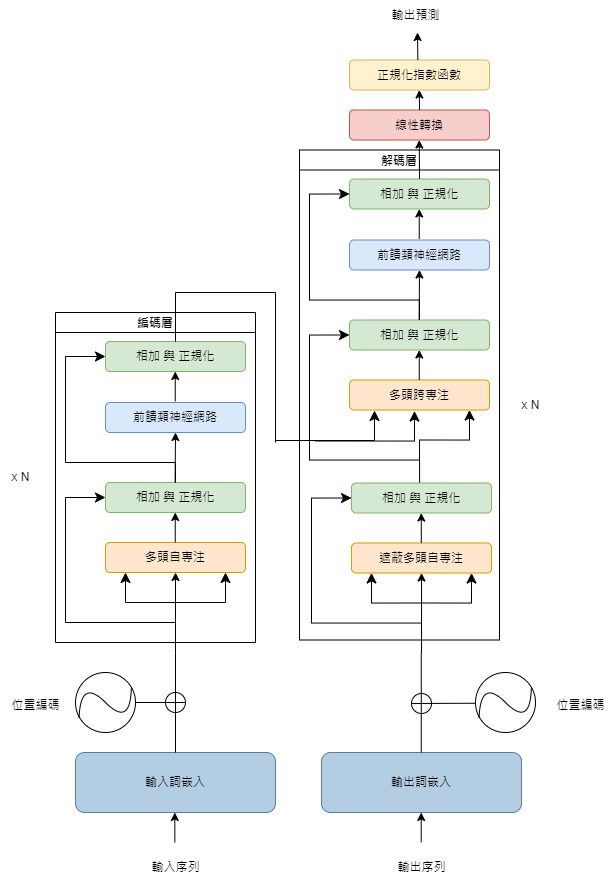
\includegraphics[width=0.5\linewidth]{figures/tfm_arch.drawio.png}
    \caption{轉換器架構圖}
    \label{fig:tfm_arch}
\end{figure}

由於轉換器不需對每個時間點一一運算,使其得以實現高度平行化的優勢,類神經網路得以透過專注機制的幫助同時進行序列資料的大量訓練,這種可擴展性(Scalability)因而在自然語言和語音處理都獲得了巨大的進展,近乎取代了原先遞迴式類神經網路的應用場景,近年甚至被電腦視覺的研究者推廣應用在圖像類的資料上 \cite{dosovitskiy2021image},足以展現此種模型架構的彈性與泛用性,是目前最前沿人工智慧的主流架構。

除了模型架構,機器學習中不可或缺的另一大部分即是對資料的編碼過程。如何更有效率的讓機器可以理解、處理和輸出,是機器學習乃至深層學習的一大課題。面對捉摸不定、抽象且變化萬千的人類語言,語音和文字處理如何對資料去蕪存菁,表徵學習更是重中之重。

\section{表徵與自監督式學習}

\subsection{特徵抽取與表徵學習 }
  
不論採用何種模型,為了讓機器可以處理並捕捉輸入資料中的訊號與模式(Pattern),如何對資料編碼和運算的步驟,在機器學習稱之為特徵抽取(Feature Extraction)或表徵學習(Representation Learning),是模型建構時不可或缺的重要步驟。

對於抽象的語言概念,早期工程領域根據對語音和文字的理解,分別進行了不同的處理。對離散因而可以一個一個計數的文字,人們使用詞頻統計衍生出如 n 連詞(n-gram)、TF-IDF(Term-Frequency Inverse Document Frequncy)等特徵當成模型學習的前處理步驟;而對於連續又複雜的語音,工程師則是透過聲學原理與訊號處理的知識,使用如濾波器組(Filter Bank)、梅爾倒頻譜係數(Mel-Frequency Cepstrum Coefficient,MFCC)等特徵,當成人耳捕捉語音訊號過程之類比。

在深層學習逐漸發展的過程中,自然語言處理領域的一大里程碑,是米氏(Mikolov)提出的「word2vec」模型 \cite{mikolov_efficient_2013},以連續的向量表徵(Vector Representation)取代稀疏(Sparse)的統計數據,對離散的文字單詞進行「詞嵌入(Word Embedding)」編碼,並透過大量的文本運算,將各單詞之間的共現(Collocation)以跳躍詞(Skip-gram)、連續詞袋(Continuous Bag-of-Word,CBOW) 等演算法轉換成高維向量空間中的點,找出每個單詞最適合的語義表徵。爾後,為了更細緻的捕捉同一單詞在不同句子中可能的脈絡變化,ELMo(Embeddings from Language Model)\cite{peters_deep_2018} 提出了「脈絡化詞嵌入(Contextualized Embedding)」的概念,使得各個單詞在運算出表徵的過程可以根據上下文進行些微調整。

\subsection{自監督學習}
  
隨著轉換器模型的提出後,BERT(來自轉換器的雙向編碼器表徵,Bidirectional Encoder Representations from Transformers)\cite{devlin_bert_2019} 被提出,從大量的文本與自專注機制之中,工程師們便可不藉由人工標記,透過預先設定任務(Pretext Task)的引導,使得模型可以自己從大量文本中自行找出更細緻且考量脈絡(Contextualized)的語義關係,並在許多文字的任務上獲得了超越以往的成績。

自此,楊氏(Yann LeCun)將此種以特定的任務作為引導,藉助資料本身的結構替代標註,以從大量的未標註資料中進行學習資料模式(Pattren)訓練方式,被稱之為「自監督學習(Self-supervised Learning,SSL)」。BERT 的成功使得自監督學習自此大行其道,並出現了許多由巨量資料進行預訓練(Pre-train)而成的基石模型(Foundation Model),很好的解決在語言處理領域中資料飢餓(Data Hungry)的問題。此後人們在解決語言相關任務時,便不需要從頭蒐集資料與進行耗時耗能的訓練過程,而是可以透過基石模型優良的泛化(Generalization)能力,找出對應各種應用任務的資訊予以解決。相比於預訓練的任務,這些更貼近日常現實的任務被稱為「下游任務(Downstream Task)」,而可以應對廣泛的下游任務種類,則是這些基石模型最大的優勢。

有鑑於文字處理方面的成功,語音領域的研究者便嘗試將相似的模式套用於語音之上,眾多語音基石模型也隨之出現。因為大量的語音資料庫本身,可以幫助模型去萃取出有助於下游任務的語音表徵(Speech Representation),並在各式任務上獲得了超越傳統聲學特徵的表現。由於語音表徵具備的無窮潛力,已經逐漸成為聲學特徵以外,用來處理語音訊號時的新選擇。

依照這些語音自監督模型在預訓練的學習模式,大致可以分為重建式、預測式與對比式模型,以下分別按照這三類模式介紹這些語音基石模型:

\subsubsection{重建式學習(Reconstruction Learning)}

此類模型藉由對輸入訊號進行擾動(Perturb)後,期望模型將被更動的輸入重新預測回原始的資料,通常減損函數表示為:

$$\mathcal{L}_{recon} = \mathbb{E}_x[|f_\theta(\tilde{x}) - x|]$$

其中 $\tilde{x}$ 為 $x$ 擾動後的資料,$f_\theta(\cdot)$ 為模型代表的函數。擾動的方式可能以遮蔽為主要方式,在文字處理以 BERT 為代表, 因此又被稱為「遮蔽語言模型(Masked Language Model,MLM)」。在語音中採用此方式學習的有 Mockingjay \cite{liu_mockingjay_2019}、TERA \cite{t_tera_2021} 等模型。  % NPC

\subsubsection{預測式學習(Predictive Learning)}

這類模型透過預訂一些學習目標的函數,製造類似輸入與輸出的配對資料,讓模型去預測該函數的結果,來學習資料中的特定結構。其訓練減損函數可表示為:

$$\mathcal{L}_{pred} = \mathbb{E}_x[\text{eval}(f_\theta(x), \hat{f}(x))]$$

其中 $\hat{f}$ 是期望模型學習到的目標函數,$f_\theta(\cdot)$ 為模型代表的函數,$\text{eval}$ 則是用以評估此預測好壞的標準。

目標函數最典型的代表是單純的自迴歸(Auto-regressive),也就是期望模型可以預測未來時間點的輸入表徵。文字方面以生成式預訓練轉換器(Generative Pretrained Transformer,GPT\cite{radford_language_nodate, brown_language_2020})系列為代表,而語音上的 APC \cite{chung_generative_2020} 也是採用此種模式。

此外,語音基石模型還可以使用其他的訓練目標,如 PASE+ \cite{ravanelli_multi-task_2020} 要求模型得以預測他種模型的表徵,而本文著重探究的隱藏單元 BERT(Hidden-unit BERT,HuBERT)\cite{hsu_hubert_2021, hsu_hubert_2021-2}, 則是以預測輸入表徵進行分群(Cluster)後的結果。HuBERT 預測的目標又被視為偽標註(Pseudo-label),在後面將特別細究相關內容。

\subsubsection{對比式學習(Contrastive Learning)}

這種學習方式的訓練目標是要求模型區分正樣本(Positive Sample)與負樣本(Negative Sample)的差異,減損函數通常定義為:

$$\mathcal{L}_{contr} = -\mathbb{E}_x\left[\log
\left(
{\frac
{\sum_{\tilde{x} \in x_{pos}}\exp(\text{sim}(x, \tilde{x}))}
{\sum_{\tilde{x} \in \mathcal{X}}\exp(\text{sim}(x, \tilde{x}))}
}\right)\right]$$

其中 $x$ 為輸入,$x_{pos}$ 為正樣本,$\mathcal{X}$ 為整個包含正負樣本的資料集;$\text{sim}(\cdot, \cdot)$ 是評估兩個樣本之間相似程度的函數,最常使用的相似度函數為內積運算得出的餘弦相似度(Cosine Similarity)。語音上最早使用對比式學習的模型為對比預測編碼(Contrastive Predictive Coding,CPC)\cite{maekaku2022speech},之後如 Wav2vec \cite{schneider2019wav2vec}、Modified CPC \cite{rivière2020unsupervised}、Wav2vec 2.0 \cite{baevski2020wav2vec} 等等模型亦是以對比正負樣本的模式訓練,只是訓練時正負樣本的定義有差異,如 Wav2vec 僅以時間維度上相同的向量為正樣本,其餘則以固定一段時間內的向量皆為正樣本。

對比式學習藉由正負樣本的定義,將預訓練任務形塑成分類問題,因此減損函數本質上為交叉熵(Cross-Entropy),使模型可以將訓練資料中的結構差異判斷出來。

\subsection{向量量化與離散單元}

語音訊號雖然本身記錄的是語言的資訊,然而卻和影像資料一樣都是連續數值的資料,不像離散的文字相較之下易與處,因而發展出了許多應用廣泛的模型。為了使語音模型的訓練可以套用自然語言處理領域的演算法,從連續語音中找出離散的表徵因而逐漸發展起來,而這類研究又被稱為「聲學單元發掘(Acoustic Unit Discovery,AUD)」。

由於語言概念本質上是有離散符號的,因此向量量化的技術常被用在學習需要涉及語言標註的情境之下,如電腦視覺經典的量化向量變分自編碼器(Vector-Quantized Variational Autoencoder,VQ-VAE)\cite{van2017neural},便是利用影像標註是離散語言單詞的特性,使得模型學習出來的表徵向量被約束在編碼簿(Codebook) 的幾個向量之中。

% 將模型的連續特徵透過甘式軟性最大化和 K-平均兩種向量量化技術
在語音的領域,基於 Wav2vec 之上,Vq-wav2vec \cite{baevski2019vq} 和 Wav2vec 2.0 將連續的語音特徵量化加入訓練的目標中,在語音辨識等任務上獲得了不少的進步。

HuBERT 則是應用事先對連續的 MFCC 特徵進行 K-平均(K-Means)演算法分群後,以所得的群心(Centroid)編號作為訓練目標,實施類似文字 BERT 的遮蔽語言模型訓練,並將第一次訓練得到的語音表徵再次分群後替代 MFCC 特徵再次訓練。這些經過兩輪訓練後,從模型表徵分群得到的群心即被視為「隱藏單元(Hidden Unit)」,編碼了語音訊號中較為代表性的若干個聲學特徵。而透過找出隱藏單元的過程,HuBERT 可以在低資源的情形下達到與 Wav2vec 2.0 接近的語音辨識成績。

\subsection{離散單元與無文字(Textless)架構}

奠基於 HuBERT 等語音基石模型的成功,Meta 利用隱藏單元的想法,將大量的語音資料表徵進行 K-平均演算法,作為這些語音訊號的偽標籤。如此得到的大量離散隱藏單元便形成了形同「偽文字(Pseudo-text)」的語料庫,於是他們基於這些離散單元作為文字訓練語言模型,稱為「生成式口語語言模型(Generative Spoken Language Model,GSLM)」。配合反向以語音合成的方式訓練一個基於離散單元的語音生成模型,整體架構便能完全不依賴文字標註,就訓練出一個純語音的語言模型,因而被稱為「無文字(Textless)架構」\cite{noauthor_textless_2021}。

無文字的模式目前在語音問答(Spoken Question Answering)\cite{lin2022dual} 跟語音到語音翻譯 \cite{chen_speech--speech_2023} 獲得了前所未有的進展。自此這類「離散單元(Discrete Unit)」被視為一項類似文字卻不需要真的依賴人類文字標記的語音表徵,以儲存所需的位元率(Bit Rate)較低與可以套用文字的「語言模型」之訓練模式作為最大優勢為語音社群廣泛借鑑,後續也出現了許多如 \cite{zhang2024speechtokenizer} 等等嘗試將語音以離散表徵編碼的研究。

然而,雖然在系統與應用任務上獲得了很大的成功,但這些離散單元本身究竟與文字存在多少差異,或能夠多少的幫助語音語言模型的訓練與建立,仍然是目前本領域探討的焦點議題。有鑑於此,本論文基於語言知識,從最接近文字但又跟語音訊號最密切相關的「音位(Phoneme)」開始探討,期望對離散單元本身究竟能夠帶給我們什麼特徵、如何幫助後續應用進行進一步的研究。

\section{本章節總結}

本章節先是對深層學習模型的核心部件 --- 類神經網路進行了基本原理的介紹,其後對本論文研究的核心 --- 「語音表徵」與「離散單元」的發展演進與歷史進行了簡單的梳理。此後兩章節就會緊扣著這些基石模型得到的離散特徵,將其與尤其是「音位」這類語音學標記之間的統計關係進行更進一步的分析。
